% Euclidean Handout Number six
\documentclass{tufte-handout}

%\geometry{showframe}% for debugging purposes -- displays the margins

%%%% Packages to make things pretty
\usepackage{amsmath,amsthm}
\usepackage{booktabs}
\usepackage{graphicx}
\setkeys{Gin}{width=\linewidth,totalheight=\textheight,keepaspectratio}
\graphicspath{{graphics/}}
\usepackage{units}
\usepackage{fancyvrb}
\fvset{fontsize=\normalsize}
\usepackage{multicol}
\usepackage{pdfpages}

%%%% Theorem Evironments
\theoremstyle{definition}
\swapnumbers
\newtheorem{problem}{Problem}[section]
\newtheorem{conjecture}[problem]{Conjecture}
\newtheorem*{definition}{Definition}
\newtheorem*{theorem}{Theorem}
\newtheorem{question}[problem]{Question}
\newtheorem{challenge}[problem]{Challenge}
\newtheorem*{postulate}{Postulate}

%%%%%

\title{Euclidean Geometry:\\An Introduction to Mathematical Work}
\author[Math 3600]{Math 3600}
\date{Spring 2017}

\begin{document}

\maketitle

\begin{marginfigure}
    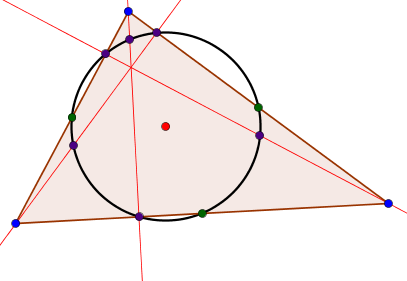
\includegraphics{NPC}
\end{marginfigure}

\setcounter{section}{6}
\section{Regular Figures, A Warm-up}

A great part of the allure of geometry is figures with symmetry. Inspired by this, let us study some polygons that have a lot of symmetry.

\begin{definition}\label{defn:regular}
A polygon is said to be \emph{equilateral} if all of its sides are congruent, \emph{equiangular} if all of its angles are congruent, and \emph{regular} if it is both equilateral and equiangular.
\end{definition}

\begin{conjecture}\label{conj:equilateral-triangle}
An equilateral triangle is equiangular, hence regular.
\end{conjecture}

\begin{conjecture}\label{conj:regular-rhombus}
Let $ABCD$ be a rhombus. If angle $A$ is congruent to $B$, then $ABCD$ is regular.
\end{conjecture}

\begin{definition}[reminder]\label{defn:square}
A regular quadrilateral is called a \emph{square}.
\end{definition}


\begin{problem}\label{prob:equilateral-quad}
Does Conjecture \ref{conj:regular-rhombus} hold if we replace ``angle $B$'' by ``angle $C$''? State a result and prove it.
\end{problem}

\begin{conjecture}\label{conj:equilateral-pentagon}
Let $ABCDE$ be an equilateral pentagon. If angle $A$ is congruent to angle $B$, then $ABCDE$ is regular.
\end{conjecture}



\begin{conjecture}\label{conj:regular-pentagon-central-triangle}
Let $ABCDE$ be a regular pentagon. The triangle $ACD$ is isosceles.
\end{conjecture}

\begin{problem}\label{prob:reg-pentagon-angles}
Let $ABCDE$ be a regular pentagon. State the relationship between the angles $CAD$ and $ACD$ that shows how special the triangle is. Prove your observation.
\end{problem}

\begin{problem}\label{prob:reg-pentagon-types}
Find experimental evidence for the number of regular pentagons with a given side. (Try using five toothpicks!)\\[.1in]
\end{problem}





\end{document}
